\chapter{Report delle vendite}
\label{cap:report-vendite}

\intro{In questo capitolo, vengono descritte le teorie e le tecniche utilizzate per l'analisi delle vendite, con particolare attenzione all'elaborazione dei dati, alle tecniche di analisi utilizzate e ai grafici generati. Viene inoltre discusso il beneficio dell'automazione dell'analisi delle vendite in confronto all'alternativa manuale.}


\section{Benefici dell’automazione dell’analisi delle vendite}

La \gls{busintel} è un insieme di tecnologie e pratiche che consentono alle aziende di raccogliere, analizzare e presentare dati per supportare il processo decisionale. L'automazione dell'analisi delle vendite rappresenta un passo avanti significativo rispetto all'analisi manuale, offrendo numerosi vantaggi:
\begin{itemize}
    \item \textbf{Efficienza}: l'automazione consente di elaborare grandi volumi di dati in tempi ridotti, riducendo il tempo necessario per generare report e analisi;
    \item \textbf{Accuratezza}: le operazioni automatizzate riducono il rischio di errori umani, garantendo risultati più precisi e affidabili;
    \item \textbf{Scalabilità}: le soluzioni automatizzate possono gestire facilmente l'aumento dei dati e delle richieste di analisi, adattandosi alle esigenze aziendali in crescita;
    \item \textbf{Accessibilità}: i report automatizzati possono essere facilmente condivisi tra i membri del team e le parti interessate, migliorando la collaborazione e la comunicazione;
    \item \textbf{Personalizzazione}: le soluzioni automatizzate possono essere configurate per generare report specifici in base alle esigenze dell'azienda, consentendo un'analisi mirata.
\end{itemize}

Di conseguenza, compito di questo progetto è stato quello di sviluppare un sistema automatizzato per l'analisi delle vendite, in grado di generare report dettagliati e personalizzati in modo rapido ed efficiente. Questo sistema si basa su un processo di raccolta, elaborazione e visualizzazione dei dati, che consente di ottenere informazioni utili per prendere decisioni strategiche e migliorare le performance aziendali.



\section{Studio delle colonne del dataset}
\label{sec:studio-colonne-dataset}
Per poter analizzare le vendite, è fondamentale comprendere le colonne dei dataset dei quali si dispone. Inizialmente, è stato reso disponibile un unico dataset, che d'ora in poi denominerò \emph{Orders\_export}, fornito dall'azienda di e-commerce committente, dunque le colonne di questo dataset sono state studiate in dettaglio e prese come riferimento per l'analisi delle vendite e per la selezione dei successivi dataset. Le colonne originali di \emph{Orders\_export} sono le seguenti:
\begin{itemize}
    \item \textbf{Numero Ordine}: identificativo univoco dell'ordine;
    \item \textbf{Data Ordine}: data dell'ordine, che riporta anche il timestamp esatto;
    \item \textbf{ID Cliente}: identificativo univoco del cliente;
    \item \textbf{Nome Cliente}: nome del cliente;
    \item \textbf{Cognome Cliente}: cognome del cliente;
    \item \textbf{Company}: azienda del cliente, se presente;
    \item \textbf{SKU Prodotto}: codice univoco del prodotto (Stock Keeping Unit);
    \item \textbf{ID Prodotto}: identificativo univoco del prodotto;
    \item \textbf{Descrizione Prodotto}: descrizione del prodotto;
    \item \textbf{Quantità}: quantità di prodotto ordinata;
    \item \textbf{Prezzo Unitario}: prezzo unitario del prodotto;
    \item \textbf{Valore Riga}: importo totale dell'acquisto del prodotto. Ciò si deduce solo dai valori contenuti nella colonna, perchè il nominativo della stessa purtroppo non è stato attribuito in modo corretto dall'azienda committente.
\end{itemize}

Dopo un primo sguardo alle colonne, è apparsa chiara la necessità di operare un \gls{preprocessing} delle stesse, in modo da poter analizzare le vendite in modo standard ed efficace. Ne è esempio la colonna \emph{Valore Riga}, che non fa comprendere il suo contenuto subito alla prima lettura del nome, e dunque necessita di un cambio di nominativo.

Dopo aver esaminato le colonne del dataset \emph{Orders\_export}, è stato sviluppato un sistema di preprocessing, descritto più nel dettaglio a livello implementativo nella sezione \S\ref{sec:preprocessing}. In questa fase, sono state scelte le seguenti colonne per l'analisi delle vendite, e il loro nome è stato tradotto in inglese per uniformità con il resto del progetto:
\begin{itemize}
    \item \textbf{Order ID}: identificativo univoco dell'ordine;
    \item \textbf{Order Timestamp}: data e ora esatta dell'ordine;
    \item \textbf{Customer ID}: identificativo univoco del cliente;
    \item \textbf{Customer Name}: nome e cognome del cliente;
    \item \textbf{Product SKU}: codice univoco del prodotto (Stock Keeping Unit);
    \item \textbf{Product Name}: nome o descrizione del prodotto;
    \item \textbf{Unit Price}: prezzo unitario del prodotto;
    \item \textbf{Quantity}: quantità di prodotto ordinata;
    \item \textbf{Total Price}: importo totale relativo all'acquisto del prodotto.
\end{itemize}

Queste colonne sono state dunque prese come riferimento per cercare ulteriori dataset che potessero essere utili per l'analisi delle vendite. In particolare, sono stati cercati dataset pubblici nella piattaforma \gls{kaggle} che contenessero le stesse colonne o colonne riconducibili a quelle standardizzate di \emph{Orders\_export}. I dataset trovati sono stati denominati con il nome dell'utente che li ha caricati su Kaggle.

La tabella \ref{tab:dataset-riassunto} mostra tutti i dataset che sono stati utilizzati per il progetto, con il loro numero di righe, numero di clienti unici e numero di prodotti unici:
\begin{table}[h]
    \centering
    \begin{tabular}{|l|r|r|r|}
        \hline
        \multicolumn{1}{|c|}{\textbf{Dataset}} & \multicolumn{1}{|c|}{\textbf{Numero righe}} & \multicolumn{1}{|c|}{\textbf{Clienti}} & \multicolumn{1}{|c|}{\textbf{Prodotti}} \\
        \hline
        Anwer          & 51.290 & 795   & 10.292 \\
        Cornelius      & 15.000 & 14.095 & 15.000 \\
        Dee            & 2.747  & 89    & 109 \\
        Delikkaya      & 44.804 & 35.389 & 1.000 \\
        Feroze         & 250   & 10    & 10 \\
        Orders\_export & 26.862 & 23.252 & 4.114 \\
        Segura         & 2.823  & 92    & 109 \\
        Shaw           & 3.203  & 686   & 1.494 \\
        Swillm         & 50.000 & 8.157  & 47 \\
        Vaghasiya      & 5.000  & 2.172  & 268 \\
        \hline
    \end{tabular}
    \caption{Dataset utilizzati per l'analisi delle vendite, con numero di righe, clienti e prodotti.}
    \label{tab:dataset-riassunto}
\end{table}

Ogni dataset è stato dunque trattato per ottenere le stesse colonne standardizzate, in modo da poterle confrontare e analizzare in modo efficace.
Inoltre, sono state successivamente aggiunte le seguenti colonne, ricavate dalla colonna \emph{Order Timestamp}, per facilitare alcune operazioni di analisi temporale e per poter generare statistiche utili:
\begin{itemize}
    \item \textbf{Order Day}: giorno dell'ordine (1-31);
    \item \textbf{Order Week}: settimana dell'anno in cui è stato effettuato l'ordine (1-53);
    \item \textbf{Order Month}: mese in cui è stato effettuato l'ordine (1-12);
    \item \textbf{Order Year}: anno in cui è stato effettuato l'ordine (YYYY);
    \item \textbf{ISO Date}: data dell'ordine in formato ISO (YYYY-MM-DD);
    \item \textbf{ISO Month}: mese dell'ordine in formato ISO (YYYY-MM).
\end{itemize}

Fatto ciò, in parallelo con lo studio delle statistiche utili e dei grafici, si è visto necessario introdurre delle ulteriori colonne legate alla data, ma descrittive invece che numeriche, per allinearsi con il linguaggio naturale del report. Siccome il contenuto di tali colonne dipende dalla lingua del report, la loro creazione è ulteriormente descritta a livello implementativo nella sezione \S\ref{sec:language-processing}, dedicata alla gestione della lingua. Le colonne aggiuntive sono le seguenti:
\begin{itemize}
    \item \textbf{Date}: data dell'ordine in formato naturale, ad esempio "1 gennaio 2023";
    \item \textbf{Month}: mese dell'ordine in formato naturale, ad esempio "gennaio 2023";
    \item \textbf{Week}: settimana dell'anno in formato naturale, ottenuta unendo assieme le date del lunedì e della domenica di tale settimana, ad esempio "3 febbraio 2025 - 9 febbraio 2025".
\end{itemize}

A questo punto, i dataset preprocessati sono pronti per essere analizzati, e le colonne standardizzate sono pronte per essere utilizzate per ricavare le statistiche utili e i grafici.



\section{Valutazione delle statistiche utili}

Per poter analizzare le vendite, è fondamentale comprendere quali statistiche siano utili per ottenere informazioni significative. L'azienda committente, consapevole di ciò, ha fornito un esempio di report delle vendite, visibile nell'immagine \ref{fig:oribea-report-example}, che è stato utilizzato come base per la valutazione delle statistiche utili.

\begin{figure}[!h]
    \centering
    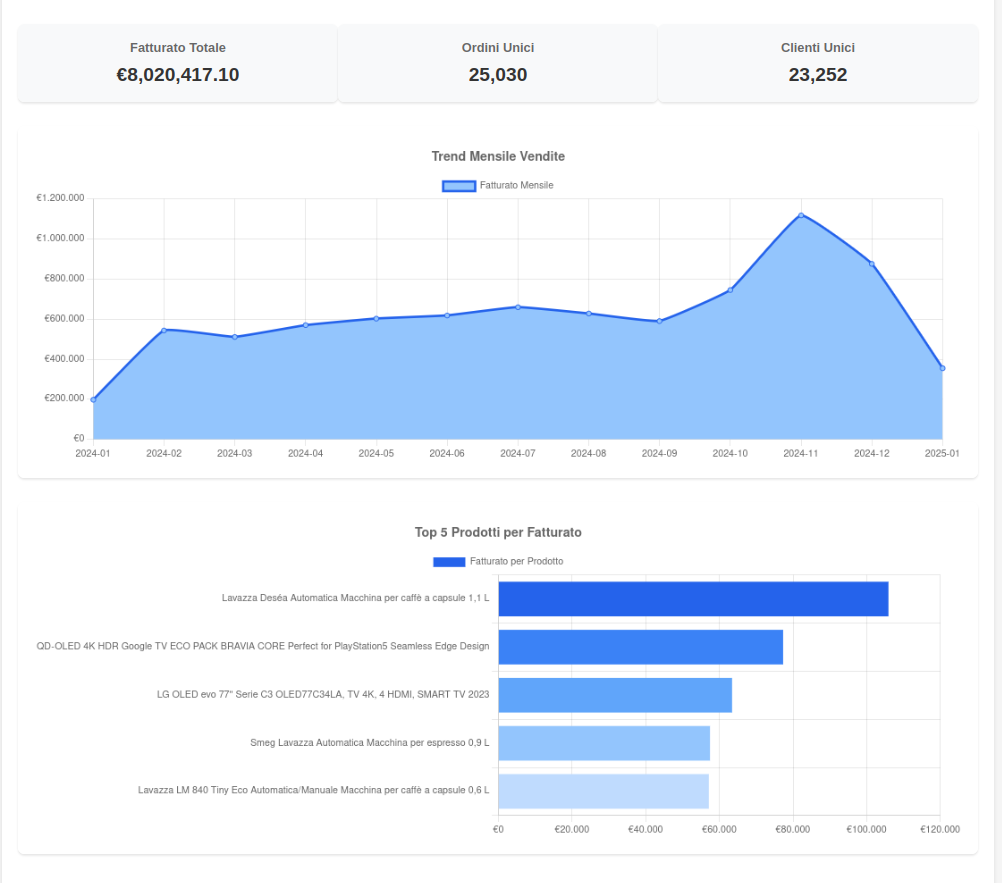
\includegraphics[width=0.9\columnwidth]{Oribea - Esempio di report delle vendite.png}
    \caption{Esempio di report delle vendite fornito da Oribea.}
    \label{fig:oribea-report-example}
\end{figure}

Il report contiene le seguenti statistiche:
\begin{itemize}
    \item \textbf{Fatturato Totale}: il totale delle vendite effettuate nel periodo racchiuso nel dataset;
    \item \textbf{Ordini Unici}: il numero di ordini unici effettuati nel periodo racchiuso nel dataset; questa statistica è necessaria perchè più righe contenenti lo stesso ordine possono essere presenti nel dataset, a causa della possibile presenza di più prodotti nello stesso ordine;
    \item \textbf{Clienti Unici}: il numero di clienti unici che hanno effettuato ordini nel periodo racchiuso nel dataset; questa statistica è necessaria perchè più righe contenenti lo stesso cliente possono essere presenti nel dataset, a causa della possibile presenza di più ordini effettuati dallo stesso cliente.
\end{itemize}

Queste statistiche sono state scelte come base per l'analisi delle vendite, e sono state implementate nel sistema di analisi automatizzato. Successivamente, sono state aggiunte altre statistiche utili, che sono state scelte in base alla loro rilevanza per l'analisi delle vendite e alla loro capacità di fornire informazioni significative. Le statistiche aggiuntive sono le seguenti:
\begin{itemize}
    \item \textbf{Prodotti Unici}: il numero di prodotti unici venduti nel periodo racchiuso nel dataset; questa statistica è necessaria perchè più righe contenenti lo stesso prodotto possono essere presenti nel dataset, a causa della presenza di più ordini effettuati dallo stesso cliente;
    \item \textbf{Spesa Media per Ordine}: la spesa media per ordine, calcolata come il fatturato totale diviso per il numero di ordini unici; questa statistica è utile per comprendere quanto i clienti spendono mediamente per ogni ordine.
\end{itemize}

Successivamente, sono state pensate delle altre elaborazioni statistiche, che però non sono state implementate nel sistema di analisi automatizzato per le ragioni spiegate nelle sezioni \S\ref{sec:recognition-brands} e \S\ref{sec:recognition-categories} riguardanti il \gls{preprocessing}.

A valle di ciò, seppure siano state pensate delle statistiche utili aggiuntive, si è deciso di non implementarle nel sistema di analisi automatizzato. Sono rimaste dunque le cinque statistiche descritte in precedenza, che sono state implementate nel sistema di analisi automatizzato e sono state utilizzate per generare il report delle vendite. Queste statistiche sono state scelte in base alla loro rilevanza per l'analisi delle vendite e alla loro capacità di fornire informazioni significative, e sono state ritenute sufficienti per ottenere un'analisi delle vendite efficace e utile.



\section{Valutazione dei grafici utili}

Per poter analizzare le vendite, è fondamentale comprendere quali grafici siano utili per ottenere informazioni significative. Nell'esempio di report delle vendite, succitato nell'immagine \ref{fig:oribea-report-example}, sono presenti anche alcuni grafici, che sono stati utilizzati come base per la valutazione dei grafici utili.
I grafici consigliati sono i seguenti:
\begin{itemize}
    \item \textbf{Trend mensile delle vendite}: un grafico a linee che mostra l'andamento delle vendite nel tempo, suddiviso per mese. Questo grafico consente di visualizzare le fluttuazioni delle vendite e di identificare eventuali tendenze stagionali;
    \item \textbf{Top 5 prodotti per fatturato}: un grafico a barre che mostra i cinque prodotti più venduti in termini di fatturato. Questo grafico consente di identificare i prodotti più popolari e redditizi.
\end{itemize}

Il report di esempio ha dunque suggerito l'utilizzo di questi due grafici, che sono stati implementati nel sistema di analisi automatizzato. Oltre a ciò, tale report ha anche suggerito le tipologie di grafici consigliate dall'azienda committente, cioè grafici a linee e a barre, che sono stati quindi scelti per il report per la loro semplicità e chiarezza nella visualizzazione dei dati.

A questo punto, sono stati pensati altri grafici utili, che sono stati implementati nel sistema di analisi automatizzato in parallelo con lo studio del colonne del dataset e con la progettazione del \gls{preprocessing}. I grafici aggiuntivi sono i seguenti:
\begin{itemize}
    \item \textbf{Top 5 clienti per spesa totale}: un grafico a barre che mostra i cinque clienti che hanno speso di più nel periodo racchiuso nel dataset. Questo grafico consente di identificare i clienti più redditizi e di valutare le strategie di fidelizzazione;
    \item \textbf{Trend mensile dei nuovi clienti}: un grafico a linee che mostra l'andamento del numero di nuovi clienti acquisiti nel tempo, suddiviso per mese. Questo grafico consente di valutare l'efficacia delle strategie di marketing e di acquisizione clienti;
    \item \textbf{Trend mennsile della percentuale di nuovi clienti}: un grafico a linee che mostra l'andamento della percentuale di nuovi clienti rispetto al totale dei clienti nel tempo, suddiviso per mese. Questo grafico consente di valutare l'efficacia delle strategie di marketing e di acquisizione clienti in relazione al numero totale di clienti; il valore della percentuale del primo mese è ovviamente 100\%, poiché il numero di nuovi clienti è uguale al numero totale di clienti fino ad allora;
    \item \textbf{Top 5 date per fatturato}: un grafico a barre che mostra le cinque date in cui si è registrato il fatturato più alto. Questo grafico consente di identificare le date più redditizie e di valutare l'efficacia delle strategie di vendita;
    \item \textbf{Top 5 settimane per fatturato}: un grafico a barre che mostra le cinque settimane in cui si è registrato il fatturato più alto. Questo grafico consente di identificare le settimane più redditizie e di valutare l'efficacia delle strategie di vendita.
\end{itemize}

Si può notare come sono stati scelti grafici prevalentemente legati al fatturato, e non a valori discreti come "quantità" o "numero" di prodotti/ordini, poiché il fatturato è stata considerata la metrica più importante per l'azienda e quella che fornisce le informazioni più significative. Al contrario, grafici legati a "quantità" o "numero" di prodotti/ordini non sono stati implementati poiché non sono stati ritenuti utili per l'analisi delle vendite.

Molti grafici scelti sono stati legati alla data, poiché si è ritenuto che l'analisi temporale delle vendite fosse fondamentale per comprendere le tendenze e le fluttuazioni delle stesse nel tempo. Da ciò si spiegano le operazioni contemporanee di aggiunta di nuove colonne legate alla data, descritte sopra nella sezione \S\ref{sec:studio-colonne-dataset}.

Infine, i sette grafici implementati nel sistema di analisi automatizzato, scelti in base alla loro rilevanza per l'analisi delle vendite e alla loro capacità di fornire informazioni significative, sono stati dunque ritenuti sufficienti per ottenere un'analisi delle vendite efficace e utile.

